% 6-8 pages !
% Propose and substantiate managerial, business and organisational solutions to the key problem(s):
% Proposals shall be prospective aiming at providing robust solutions to address the key problem(s).
% Remember to discuss the implementation aspect of your solution(s).
% There must be a coherence between the key problem(s), its causes and the proposed solutions.
% It is crucial to develop various alternative proposals for solutions. Select and motivate which proposals you think would best address the key problem.
% Use models and theories to support your proposals addressing organisational changes, changes of business model etc.

\subsection{Reworking the marketing strategy - Nipun}

Marketing strategy is a long-term, forward-looking approach with the fundamental goal of achieving a sustainable competitive advantage. [1] By analyzing the Star Model ,Business Canvas Model and Porters generic strategies we found some problems which could be improved by changing the current marketing strategy of HOWDY , which may lead the customers to onboard HOWDY to a greater extend.

Analyzing all the informations which are given to us, we made some assumptions on which we studied and structured some solutions which are given bellow-

Establish an Effective sales and Marketing team : According to the results from the previously sections, it has been already identified that the company’s current sales team is inefficient and from the company presentation[2, s.11] it was revealed that daily tasks intervene with strategy meetings. This may lead to why the company is losing money from the past years. So HOWDY can establish a strong sales and marketing team by recruiting some efficient personnel who will continuously monitor the sales progress and implement the correct and fruitful marketing strategy for the betterment of the organization. A strong Sales and Marketing team is responsible for researching and developing marketing opportunities and planning and implementing new sales plans. The Sales and Marketing Manager will also manage both the marketing and the sales staff and will perform managerial duties to meet the company's operations goals.

Put more efforts in advertising HOWDY: From analyzing previous data we can see that HOWDY is advertising their product in a limited way through their partners (Insurance companies). But it is a clear threat to their profit margin. The more they advertise HOWDY the more they will get benefit. As they have limitations in advertising through their partner’s they can find some other ways to advertise their products.

- Use LinkedIn the right way- As HOWDY is a B2B IT based organization, keeping a connection in LinkedIn will let them to be connected with other Business organizations as a lot of IT professionals, whose main target of B2B IT companies, are active on LinkedIn. HOWDY can reach a large audience by introducing a strong profile of their business through LinkedIn.

- Use Email Marketing- Email marketing is still a very effective marketing tactic with a relatively low cost and high ROI. Through Email marketing HOWDY can educate it’s audience about the products or services it can also invite the audience to attend offline events or webinars.

Introduce free Workshops and Webinars – As people love new learning experiences HOWDY can introduce some workshops or webinars related to it’s products or services. And many business organizations may get attracted to onboarding HOWDY for the wellbeing of their employee’s.

Analyze the Data and Survey- To fix HOWDYs nonproductive marketing efforts, they must first identify the problem areas. Utilize an analytical tool to determine the aspects of their strategy that aren’t working and show which marketing channels are bringing in the bulk of traffic and which aren’t. They may also implement surveys to see how customers are finding their business. Once they have this information, you can use it to their advantage
 
\subsection{Organisational restructuring - Kasper}
In order for Howdy to divert from their current path and grow their business a change in the organizational structure will benefit them greatly.

\noindent As mentioned in the previous section the marketing and sales of the company would improve by expanding the sales team.

\noindent Howdy also has the problem of the development being interrupted by day-to-day tasks like maintenance. As the development is of significant importance it would benefit Howdy to address this problem.\\
\noindent One way of doing this is by expanding the maintenance team until the workload does not surpass the resources of the team.\\
\noindent If expanding the team is not possible then another option could be to assign someone working with development to the maintenance team. This will slow the development but the continuous operation of the company is more important and then the rest of the developers will be able to completely focus on their tasks. As the workload of the maintenance might change every day the people previously from development can support the developers when the workload is small.

\noindent Even though the cost of Howdys´ product is not identified as a problem in the retrospective analysis it could still increase resources for solutions to the problems presented in this document or other activities. One of the significant costs for Howdy is the external psychologists they hire as part of their product. It is not known what the workload for this task is but hiring their own psychologists could reduce costs as an internal psychologist costs 50\% of what an external one does.

%%
%% Reworking the pricing system
%%   -- Jesper --
%%
\subsection{Reworking the pricing system - Jesper}
The key to a perfect pricing system shares information to the customer to help them decide which product to chose. A pricing table must share the right amount of information without sharing too much as this often will result in chaotic pricing tables. Our proposed pricing table solution for Howdy can be seen on [Figure \ref{pricingtable}] below.

\begin{figure}[H]
\centering
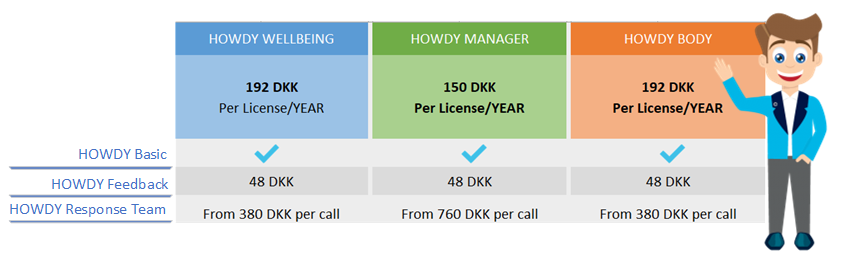
\includegraphics[scale=0.72]{figures/pricing_Howdy.png}
\caption{Howdys´ new pricing table}
\label{pricingtable}
\end{figure}

